\newpage
\section{Ομαδοποίηση}
\subsection{Εισαγωγή στην ομαδοποίηση}
Η ενότητα αυτή αφορά τους αλγορίθμους ομαδοποίησης(\textlatin{clustering}). Η δουλειά των
αλγορίθμων αυτών είναι να χωρίσουν το σύνολο των δεδομένων σε ομάδες τέτοιες ώστε τα δεδομένα μιας
ομάδας να εμφανίζουν περισσότερες ομοιότητες μεταξύ τους από ότι με τα δεδομένα των άλλων ομάδων.
Αυτός είναι και ο βασικός στόχος της διερευνητικής και στατιστικής ανάλυσης και χρησιμοποιείται
για\cite{wikicl}:
\begin{itemize}
    \item Αναγνώριση προτύπων
    \item Ανάλυση εικόνων
    \item Εξαγωγή πληροφορίας
    \item Συμπίεση δεδομένων
    \item Γραφικά υπολογιστών
    \item Μηχανική μάθηση
\end{itemize}
\begin{figure}[H]
    \centering
    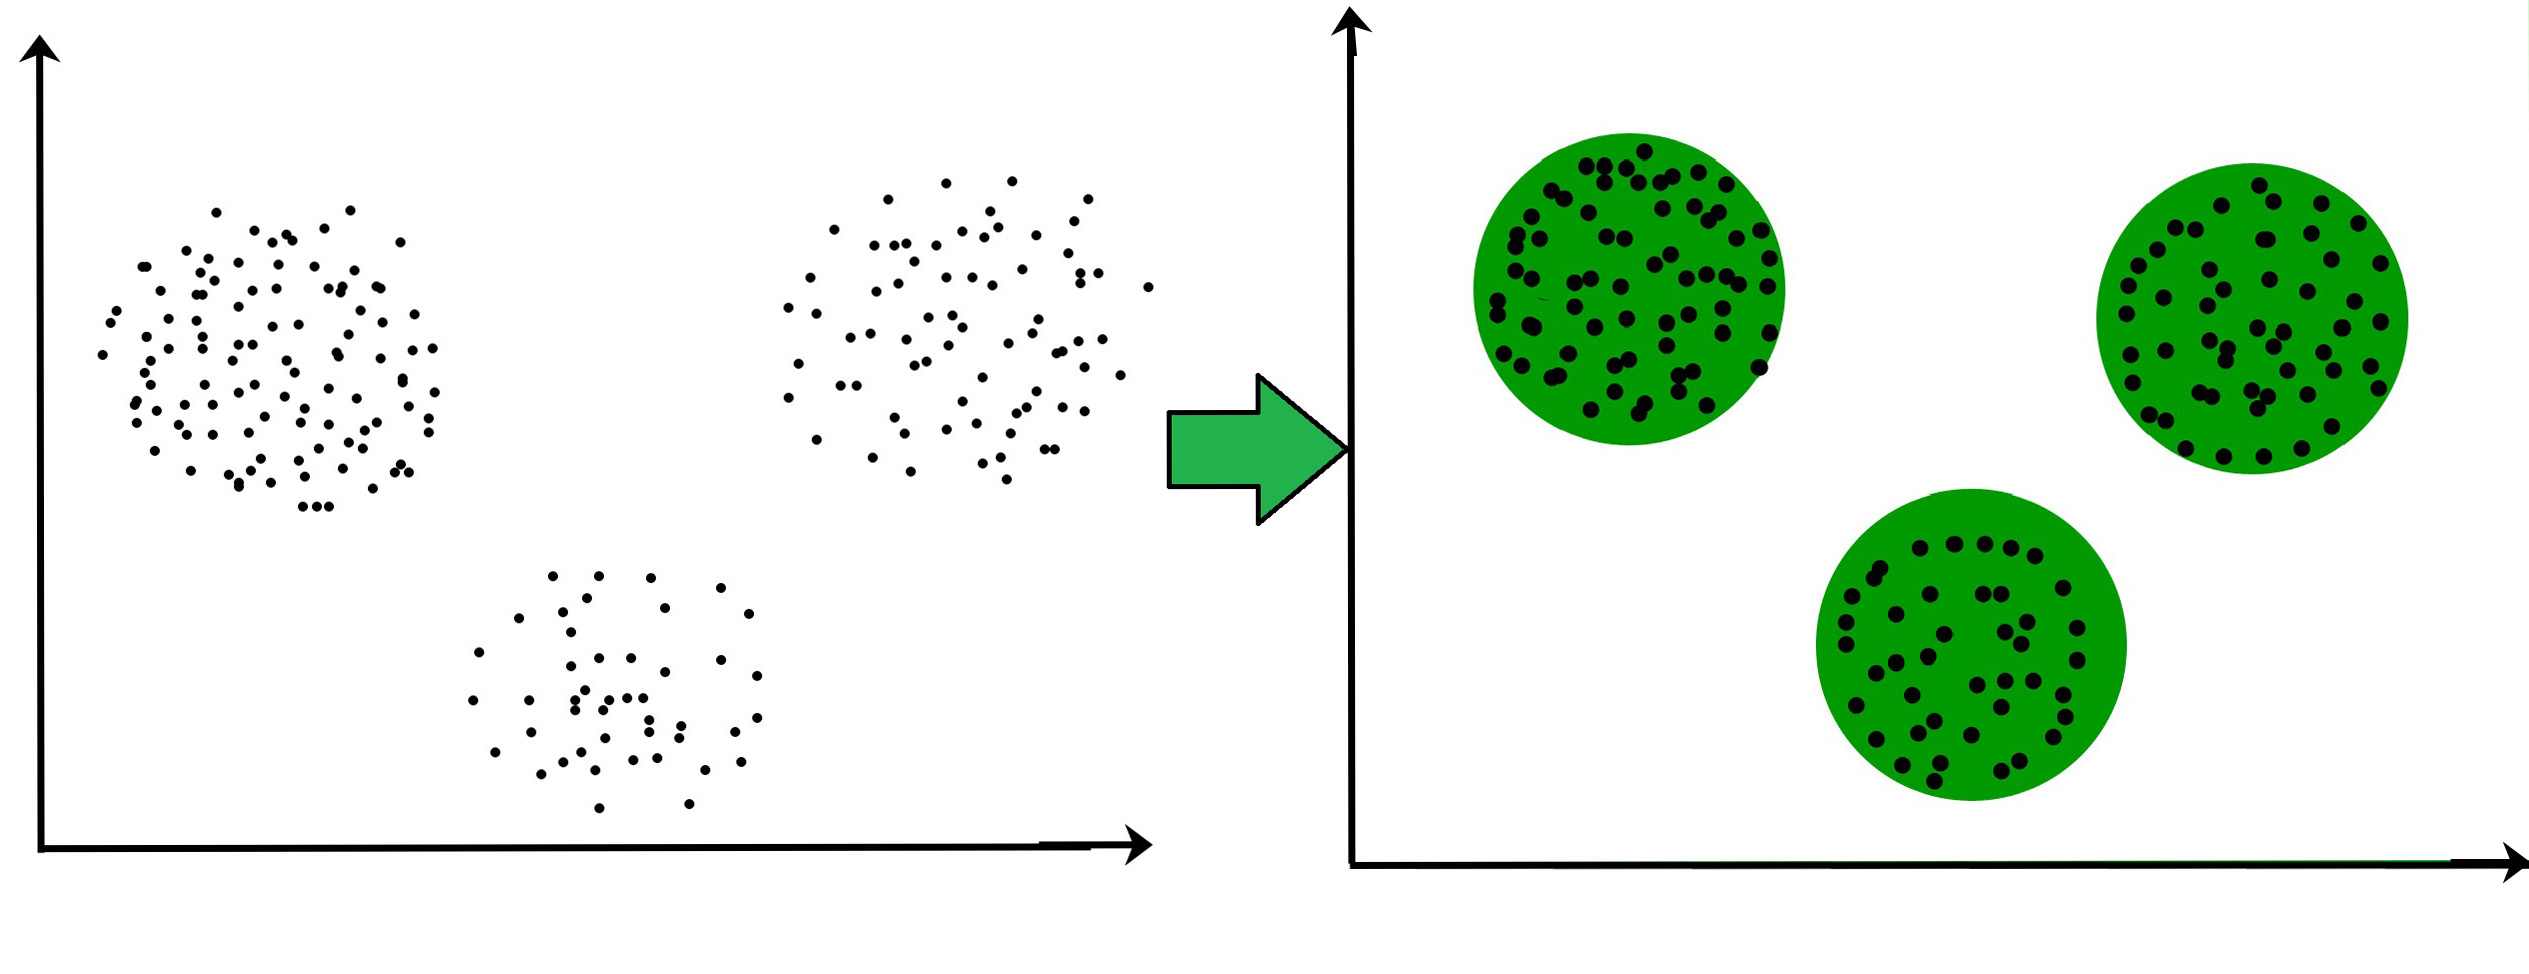
\includegraphics[width=0.7\textwidth]{images/clustering_intro.jpg}
    \caption{Γραφική αναπαράσταση ομαδοποίησης}
\end{figure}

Υπάρχουν εκατοντάδες αλγόριθμοι ομαδοποίησης οι οποίοι χρησιμοποιούν διαφορετικές μεθόδους και
τεχνικές. Δεν υπάρχει κάποιος που να υπερτερεί πλήρως των υπολοίπων αλλά η καταλληλότητα του Κάθε
αλγορίθμου εξαρτάται από το σύνολο δεδομένων. Παρά τις διαφορές τους μπορούμε να τους εντάξουμε σε
κατηγορίες συμφωνά με τον τρόπο που κάνουν την ομαδοποίηση. Οι τέσσερεις πιο βασικές κατηγορίες
είναι:
\begin{itemize}
    \item \textlatin{Centroid based clustering}
    \item \textlatin{Density based clustering}
    \item \textlatin{Distribution based clustering}
    \item \textlatin{Hierarchical clustering}
\end{itemize}
Οι κατηγορίες αυτές θα αναλυθούν περισσότερο στη συνέχεια. Επιπλέον, θα δούμε και τους πιο διάσημους αλγορίθμους που ανήκουν σε αυτές της κατηγορίες και θα αναλύσουμε και τον τρόπο
λειτουργίας τους.

\subsection{\textlatin{Centroid based clustering}}
\subsection{\textlatin{Density based clustering}}
\subsection{\textlatin{Distribution based clustering}}
\subsection{\textlatin{Hierarchical clustering}}